% !TEX root = main.tex
\section{Another Wilbur function \label{sec:other_wilbur_func}}

A new Wilbur function is adopted in Nebulas NOVA 1.0 version.

\begin{align}
\label{al:new_wilbur}
f(x) = x/(1 + (\frac{a}{x})^b) \quad a>0,0<b<1
\end{align}

\begin{figure}
\centering
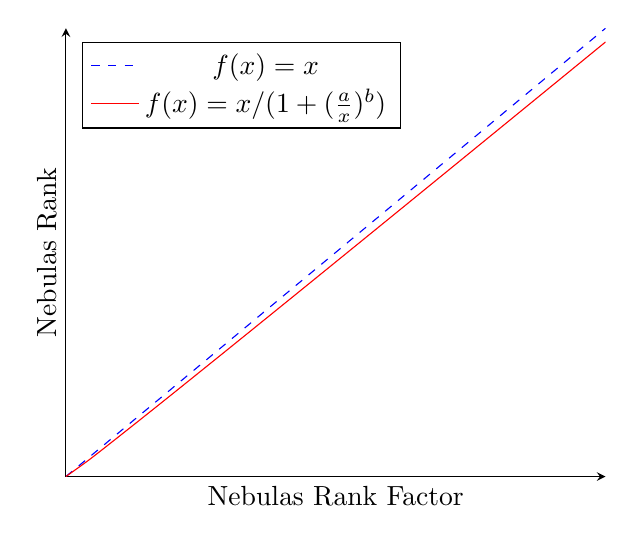
\begin{tikzpicture}[
    declare function={func(\x,\mu) = (\x / (1 + (1/\x)^(0.5)));},
    declare function={linefunc(\x) = \x;}
]
\begin{axis}[
    axis lines=left,
    enlargelimits=upper,
ticks=none,axis x line=bottom,axis y line=left,xlabel={Nebulas Rank Factor},
  ylabel={Nebulas Rank},
      legend pos=north west,
legend style={fill=none}
]
\addplot [dashed, domain=0:1000, blue] {linefunc(x)};
\addplot [smooth, domain=0:1000, red] {func(x,3)};
\addlegendentry{$f(x)=x$}
\addlegendentry{$f(x) = x/(1 + (\frac{a}{x})^b)$}
\end{axis}
\end{tikzpicture}
\caption{The curve of the Nebulas Rank function}
\label{fig:new_wilbur}
\end{figure}


As Figure \ref{fig:new_wilbur} shows, it is easy to demonstrate that the function satisfies the two properties \ref{prop:one} and \ref{prop:two} in \refsec{sec:function} as well.




